\section{Conclusion}
In this work, we presented an exploration of the functional quality of Token Merging (ToMe) for Stable Diffusion by \cite{bolya2023tomesd}. ToMe offers accelerated image generation by merging similar tokens to reduce their overall number, notably without training.\\
\\
In this thesis we conducted extensive experiments on images, obtaining speeds and fidelity superior to those of Bolya and Hoffman's default configuration.\\
ToMe has proven itself again as a practical extension to Stable Diffusion to reduce computational resources, cutting image generation time in half while mostly maintaing great image quality.\\
The application of ToMe can also be used to decrease the training time of large models, though our experiments were only concerned with improving inference.\\
\\
We hope this work can expand the understanding of Token Merging and reinforce its viability as a tool for improving the performance of diffusion models and inspire further research into the efficiency of transformers and generative models.\\



\begin{table}[!htb]
\centering
\begin{tabular}{c c c}
    
\includegraphics[width=0.3\linewidth]{static/sample_imgs/main_1x2/nepal_0.png} & 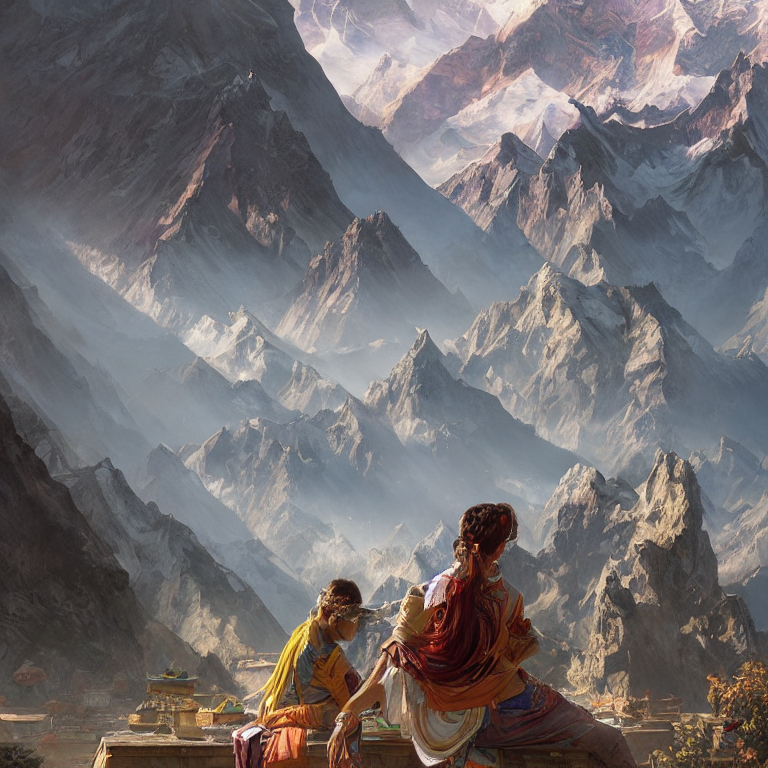
\includegraphics[width=0.3\linewidth]{static/sample_imgs/main_1x2/nepal_20.png} &
    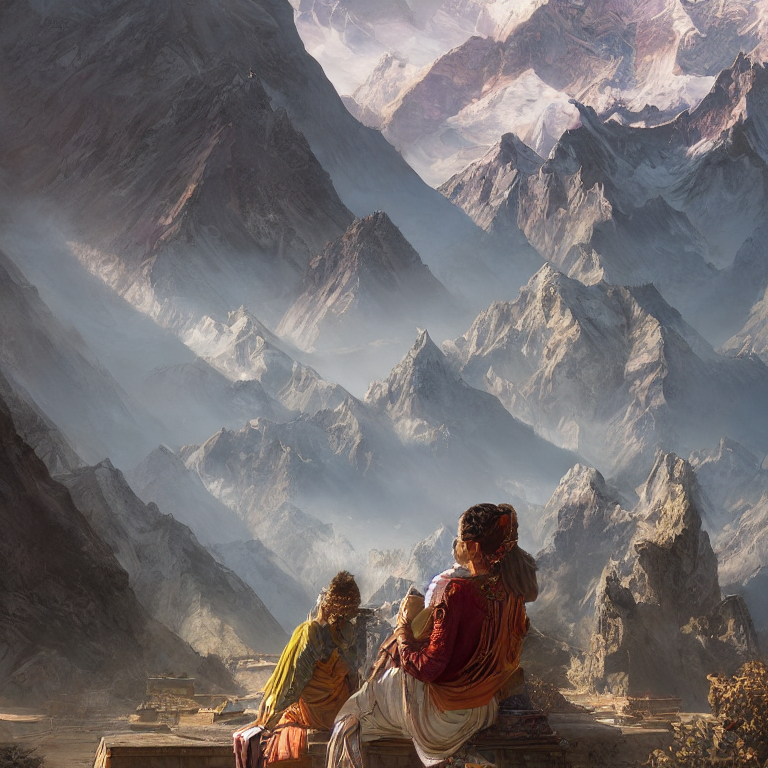
\includegraphics[width=0.3\linewidth]{static/sample_imgs/main_1x2/nepal_50.png}\\
    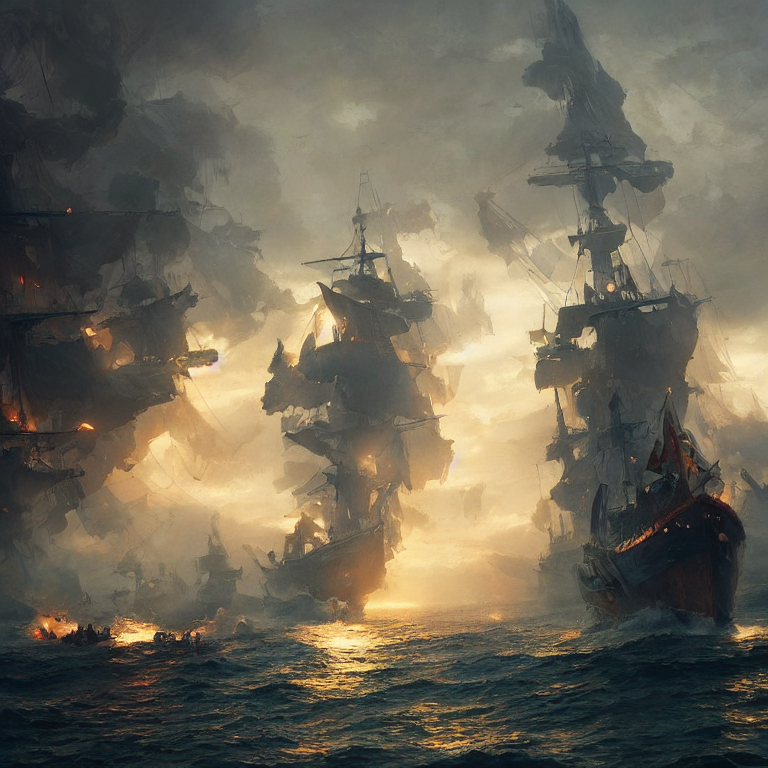
\includegraphics[width=0.3\linewidth]{static/sample_imgs/main_1x2/naval_0.png} & 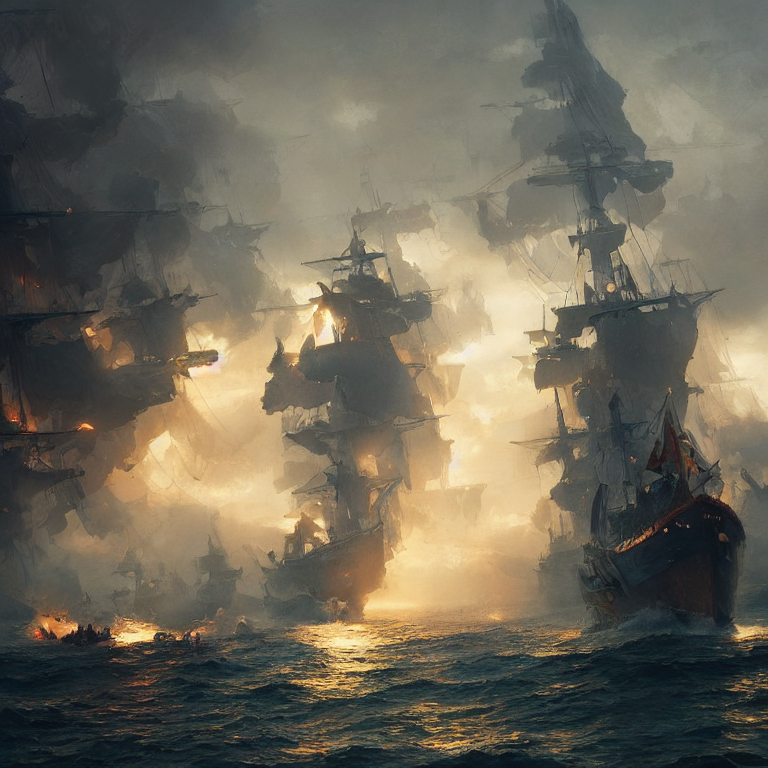
\includegraphics[width=0.3\linewidth]{static/sample_imgs/main_1x2/naval_20.png} &
    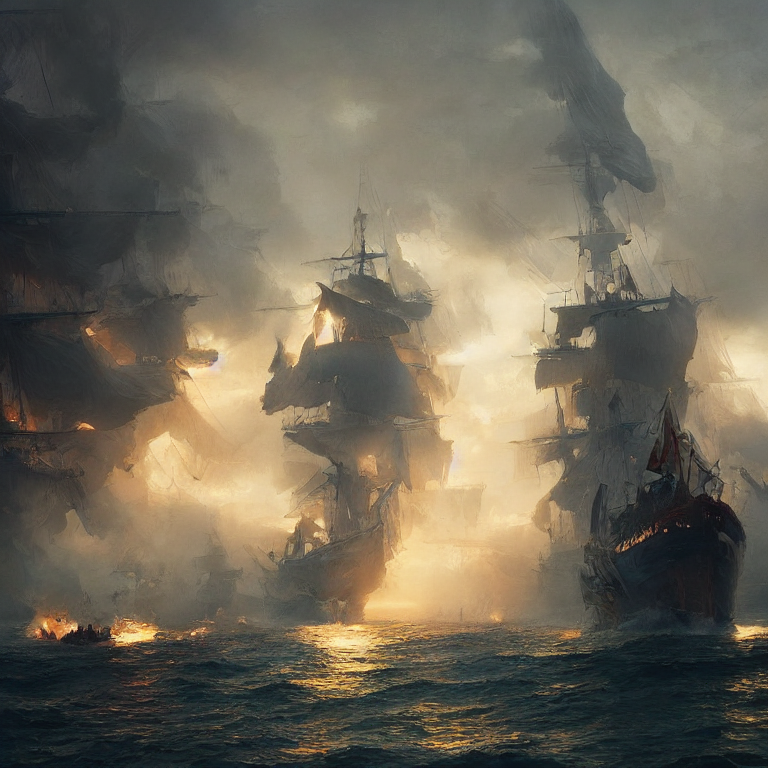
\includegraphics[width=0.3\linewidth]{static/sample_imgs/main_1x2/naval_50.png}\\
    \(r=0\%\) & \(20\%\) & \(50\%\) \\
\end{tabular}
\caption{$768 \times 768$ images created with the ToMe configured according to our best setup from \(3.2\)}
\end{table}